\begin{problem}{쓰레기}
	{standard input}{standard output}
	{2 seconds}{128 megabytes}{}
	
	
	지구이웨는 최근에 쓰레기 처리비용을 대폭 늘렸다. 이 나라가 하는 일이 다 그렇듯이 사람들이 일회용품 사용을 줄이고 쓰레기를 적게 만들 것이라는 예상과는 다르게 사람들은 길바닥에 쓰레기를 내버리기 시작했다. 폴란드의 도로들은 말 그대로 쓰레기에 파묻혀 버렸다.
	
	지구이웨의 도로망은 $n$개의 도시로 되어 있고, 몇몇 두 도시 사이에는 양방향 도로가 있다. 같은 두 도시를 잇는 도로가 두 개 이상 있지는 않다. 몇몇 도로들은 쓰레기에 파묻혀 있다.
	
	지구이웨의 정책수립자인 범수는 보복성 정책을 펼쳤다. 돈을 내고 쓰레기를 버린 사람들이 사는 도로만 청소하고, 돈을 내지 않은 사람들이 사는 도로는 청소하지 않기로 한 것이다. 점수는 이미 이 일을 하기 위해서 지도에다가 돈을 내지 않은 사람들이 사는 도로를 표시해 놓았다. 불행히도 공무원들은 그들의 계획을 이해할 수 없었지만, 단순한 지시는 이해할 수 있었다.
	
	공무원이 이해할 수 있는 지시는 쓰레기차를 몰고 어떤 한 도시에서 시작해서 다른 도로들을 쭉 방문해서 다시 원래 도시로 돌아오는 것이다. 같은 도시를 두 번 이상 방문할 경우에는 공무원들이 헛갈려서 처음 출발했던 도시를 제외하고는 두 번 이상 방문할 수 없다. 쓰레기차가 한 도로를 지날 때, 그 도로가 쓰레기에 파묻혀 있으면 그 도로를 정리하고, 그렇지 않고 깨끗하다면 그 도로에 쓰레기를 흩뿌린다.
	
	범수는 공무원이 이해할 수 있는 지시들을 통해 자신의 목적을 달성할 수 있는지가 궁금해졌다. 범수를 위해 공무원들에게 지시를 내리는 프로그램을 작성하여 주자.
	
	

	\InputFile
	
	첫째 줄에 두개의 정수 $n$, $m$이 공백 하나로 구분되어 주어진다. ($1 \le n \le 100,000$, $1 \le m \le 1,000,000$) $n$은 도시의 수 이고 $m$은 도로의 수 이다. 도시는 1부터 $n$까지 번호가 붙어 있다. 다음 $m$개의 줄에는 한 줄에 하나씩 도로들을 나타낸다. 도로들은  $a$, $b$, $s$, $t$ 가 공백 하나로 구분되어 주어진다. ($1 \le a < b \le n$, $s$, $t \in \{0,1\}$). 이것은 $a$와 $b$가 양방향 도로로 연결되어 있고, $s$는 지금 도로가 쓰레기에 파묻혀 있는지, $t$는 Zbigniew Wojna가 도로에 쓰레기를 파묻을 것인지를 의미한다. (0은 깨끗한 도로를, 1은 쓰레기에 파묻힌 도로를 의미한다.) 
	
	범수가 목적을 달성할 수 있다면, 쓰레기차가 지나야 하는 도로의 수가 총 $5\cdot m$개를 넘지 않는 지시가 존재함을 알 수 있다.
	



	\OutputFile
	
	범수의 계획에 맞는 지시들이 존재하지 않으면 ``\texttt{NIE}''를 첫째 줄에 출력한다. (따옴표는 제외한다.) 존재한다면, 도로의 갯수가 $5 \cdot m$개를 넘지 않는 공무원에게 할 지시들을 출력해야 한다. 첫째 줄에는 지시의 갯수인 $k$를 출력한다. 다음 $k$개 줄은 공무원에게 할 지시들을 출력해야 한다. $i$번째 줄에는 지시로 지나는 도로들의 수를 의미하는 $k_i$를 출력해야 한다. 이 후 공백을 출력 한 뒤, 지나야 할 도시들을 의미하는 $k_i + 1$개의 수를 공백으로 구분하여 출력해야 한다.

\SubtaskWithCost{1}{60}

\begin{itemize}
	\item $m \le 10, 000$
\end{itemize}

\SubtaskWithCost{2}{40}

추가 제한 조건이 없다.
	
	\Examples
		
	\begin{example}
	\exmp{
6 8
1 2 0 1
2 3 1 0
1 3 0 1
2 4 0 0
3 5 1 1
4 5 0 1
5 6 0 1
4 6 0 1
	}{%
2
3 1 3 2 1
3 4 6 5 4

	}%
	\end{example}
	
	\Note
	\begin{center}
	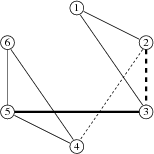
\includegraphics[]{smi.png}
	\end{center}
\end{problem}

